\documentclass[10pt]{beamer}
\usepackage{newcent}
\usepackage[utf8]{inputenc}
\usepackage[czech]{babel}
\usepackage[T1]{fontenc}
\usepackage{hyperref}
\usepackage{fancyvrb}
\usepackage{algorithmic}
\usetheme{FIT}

%%%%%%%%%%%%%%%%%%%%%%%%%%%%%%%%%%%%%%%%%%%%%%%%%%%%%%%%%%%%%%%%%%
\title[Datové struktury]{Datové struktury\,--\,Binární strom}

\author[]{Michal Blažek}

%\institute[]{Brno University of Technology, Faculty of Information Technology\\
%Bo\v{z}et\v{e}chova 1/2. 612 66 Brno - Kr\'alovo Pole\\
%xblaze38@fit.vutbr.cz}

\institute[]{Fakulta informačních technologií
Vysokého učení technického v~Brně\\
Bo\v{z}et\v{e}chova 1/2. 612 66 Brno - Kr\'alovo Pole\\
xblaze38@fit.vutbr.cz}

% České logo - Czech logo
% beamerouterthemeFIT.sty řádek 9: fitlogo1_cz

\date{\today}
%\date{} % bez data / without date

%%%%%%%%%%%%%%%%%%%%%%%%%%%%%%%%%%%%%%%%%%%%%%%%%%%%%%%%%%%%%%%%%%

\begin{document}

\frame[plain]{\titlepage}

\begin{frame}\frametitle{Co je to binární strom}

    \begin{itemize}
        \item Binární strom je orientovaný graf s~jedním vrcholem a z~něj existuje cesta do všech ostatních vrcholů grafu.
        \item Binární strom se skládá z~\emph{uzlů}, které jsou propojeny pomocí \emph{hran}.
        \item Každý uzel může mít maximálně 2 další potomky a 1 rodičovský uzel.
        \item Uzel, který nemá žádného rodiče, se nazývá \emph{kořen stromu}.
        \item Kořenový uzel existuje v~každém binárním stromě a to přesně jeden.
    \end{itemize}
    
    \begin{block}{Rekurzivní definice binárního stromu viz \cite{HonzíkJanMaxmilián1991Vkzp}:}
        \begin{quote}
            Binární strom je buď prázdný, nebo sestává z~jednoho uzlu zvaného kořen a dvou binárních podstromů – levého a pravého. (Oba podstromy mají vlastnosti binárního stromu.)
        \end{quote}
    \end{block}
    
\end{frame}

\begin{frame}\frametitle{Příklad binárního stromu}

    \begin{figure}[ht]
        \centering
        \scalebox{0.23}{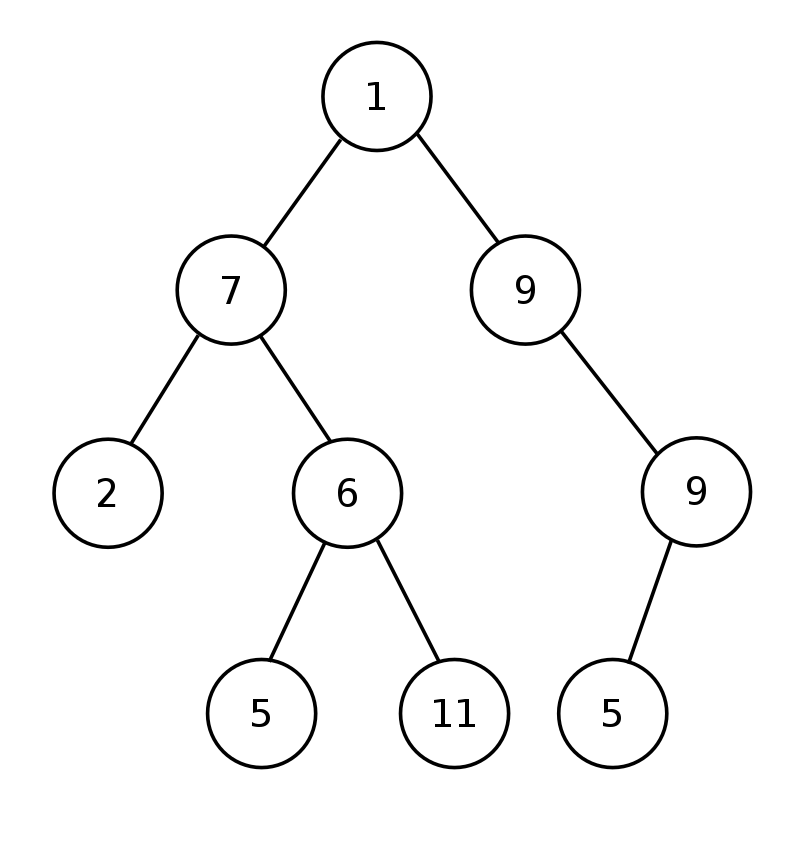
\includegraphics{img/binary_tree.png}}
        \caption{Příklad binárního stromu s~kořenem, který má hodnotu 1}
        \label{imgBinaryTree}
    \end{figure}
    
\end{frame}

\begin{frame}\frametitle{Uspořádání uzlů}

    \begin{itemize}
        \item Každý uzel má přiřazen klíč a podle něj jsou uzly uspořádány.
        \item \emph{Levý} podstrom obsahuje vždy pouze uzly s~klíčem, který je \emph{menší} než je klíč tohoto uzlu.
        \item \emph{Pravý} podstrom potom obsahuje pouze uzly s~klíčem, který je \emph{větší} než je klíč tohoto uzlu.
    \end{itemize}
    
    \begin{alertblock}{Poznámka:}
        Čísla na obrázku \ref{imgBinaryTree} nezobrazují klíče jednotlivých uzlů, ale pouze ilustrační hodnoty.
    \end{alertblock}

\end{frame}

\begin{frame}\frametitle{Výhody a nevýhody}

    \begin{block}{Výhody}
        \begin{itemize}
            \item[$+$] Ve vyváženém binárním stromě je přístup k~uzlu rychlý.
            \item[$+$] Lze využít i k~řazení prvků.
            \item[$+$] Využití při tvorbě asociativní paměti.
        \end{itemize}
    \end{block}
    
    \begin{alertblock}{Nevýhody}
        \begin{itemize}
            \item[$-$] Strom může při nešťastném vkládání a odstraňování prvků degradovat na seznam, pokud se nevyvažuje.
            \item[$-$] Vrcholy naukládají informaci o~rodiči, takže je potřeba si ukládat cestu k~danému uzlu.
        \end{itemize}
    \end{alertblock}
    
\end{frame}

\begin{frame}\frametitle{Operace}

    Základní operace:
    \begin{itemize}
        \item Průchod stromem: $O(N)$
        \item Smazání stromu: $O(N)$
        \item Přidání uzlu: $O(\log(N))$
        \item Odstranění uzlu: $O(\log(N))$
        \item Nalezení uzlu: $O(\log(N))$
    \end{itemize}
    
\end{frame}

\begin{frame}\frametitle{Průchod stromem}

    Existují 3 průchody binárním stromem:
    \begin{itemize}
        \item \emph{Preorder} - nejprve zpracovává kořen, pak levý podstrom a nakonec pravý podstrom.
        \item \emph{Inorder} - nejprve zpracovává levý podstrom, pak kořen a nakonec pravý podstrom.
        \item \emph{Postorder} - nejprve zpracovává levý podstrom, pak pravý podstrom a až nakonec kořen.
    \end{itemize}

    Toto zpracovávání se provádí rekurzivně, přičemž se vždy začíná v~kořenu binárního stromu.
    \begin{columns}
        \begin{column}{0.35\textwidth}
            \scalebox{0.15}{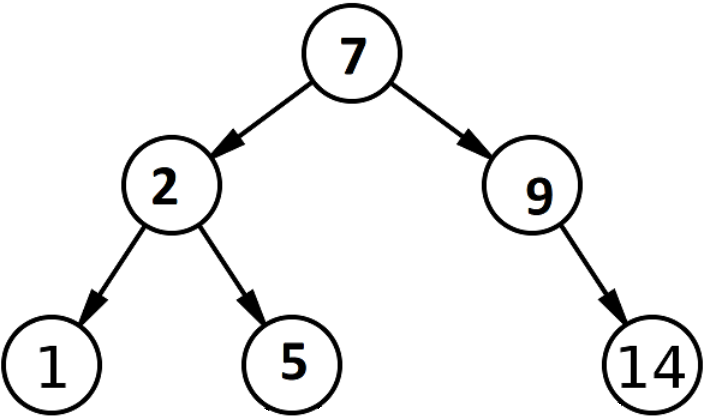
\includegraphics{img/preorder.png}}
            \label{imgPreorder}
        \end{column}
        \begin{column}{0.65\textwidth}
            \begin{itemize}
            \item Například průchod stromem na obrázku pomocí \emph{preorderu} by vypadal následovně: 7,2,1,5,9,14.
            
            \item \emph{Inorder} by nám vrátil seřazené prvky: 1,2,5,7,9,14.
            
            \item A~\emph{postorder} by vypadal následovně: 1,5,2,14,9,7
            \end{itemize}
        \end{column}
    \end{columns}
    
\end{frame}

\begin{frame}\frametitle{Pseudokódy pro průchody stromem}

    \begin{columns}
        \begin{column}{0.5\textwidth}
            void printPreorder(N* $node$):
            \begin{algorithmic}
                \IF{$node$ is not null}
                    \STATE write($node$->data)
                    \STATE printPreorder($node$->left)
                    \STATE printPreorder($node$->right)
                \ENDIF
            \end{algorithmic}
        \end{column}
        \begin{column}{0.5\textwidth}
            void printInorder(N* $node$):
            \begin{algorithmic}
                \IF{$node$ is not null}
                    \STATE printInorder($node$->left)
                    \STATE write($node$->data)
                    \STATE printInorder($node$->right)
                \ENDIF
            \end{algorithmic}
        \end{column}
    \end{columns}

    \vspace{35pt}
    
    \begin{columns}
        \begin{column}{0.5\textwidth}
            void printPostorder(N* $node$):
            \begin{algorithmic}
                \IF{$node$ is not null}
                    \STATE printPostorder($node$->left)
                    \STATE printPostorder($node$->right)
                    \STATE write($node$->data)
                \ENDIF
            \end{algorithmic}
        \end{column}
        \begin{column}{0.5\textwidth}
            \begin{block}{}
                Tyto algoritmy ukazují možnou rekurzivní implementaci jednotlivých funkcí pro průchod stromem.
            \end{block}
        \end{column}
    \end{columns}

\end{frame}

\begin{frame}\frametitle{Vyváženost}

    Pro maximální efektivitu binárního stromu je zapotřebí strom vyvážit po každém vložení nebo odstranění uzlu.
    
    Existují 2 druhy vyváženosti (lze nalézt v~\cite{HonzíkJanMaxmilián1991Vkzp}):
    \begin{itemize}
        \item \emph{Výšková} vyváženost
    \end{itemize}
    \begin{quote}
        Binární strom je \emph{výškově} vyvážený, když pro každý jeho uzel platí, že výška levého podstromu se rovná výšce pravého podstromu a nebo se liší právě o~1.
    \end{quote}
    
    \begin{itemize}
        \item \emph{Váhová} vyváženost
    \end{itemize}
    \begin{quote}
        Binární strom je \emph{váhově} vyvážený, když pro každý jeho uzel platí, že počty uzlů jeho levého a pravého podstromu se rovnají a nebo se liší právě o~1.
    \end{quote}
    
\end{frame}

\begin{frame}\frametitle{Porovnání}

    \renewcommand{\arraystretch}{2}
    \begin{table}[ht]
        \centering
        \begin{tabular}{|p{3.35cm}|p{1.8cm}|p{1.9cm}|p{1.7cm}|}
            \hline
            \textbf{Datová struktura} & \textbf{Průměrná složitost} & \textbf{Maximální složitost} & \textbf{Seřazené prvky} \\
            \hline
            Binární strom & $O(\log(N))$ & $O(\log(N))$ & Ano \\
            \hline
            Nevyvážený binární strom & $O(\log(N))$ & $O(N)$ & Ano \\
            \hline
            Vázaný seznam & $O(N)$ & $O(N)$ & Ne \\
            \hline
            Pole (nutná znalost indexu) & $O(1)$ & $O(1)$ & Ne \\
            \hline
            Hashovací tabulka & $O(1)$ & $O(N)$ & Ne \\
            \hline
        \end{tabular}
        \caption{Porovnání složitostí při hledání prvku a dalších vlastností některých datových struktur}
        \label{tabComparison}
    \end{table}
    
\end{frame}

\begin{frame}\frametitle{Reference}

    \bibliographystyle{czechiso}
    \bibliography{proj5}
    
\end{frame}

\bluepage{Děkuji za pozornost!}

\end{document}
